\documentclass{standalone}

\usepackage{tikz}

\usetikzlibrary{positioning, chains, shapes.geometric, fit, shapes, arrows.meta, calc, backgrounds}

\begin{document}

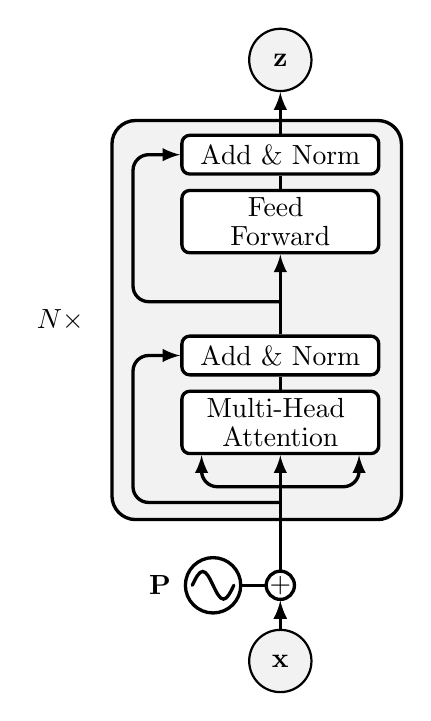
\begin{tikzpicture}[
    >=LaTeX, % Use default LaTeX arrows
    very thick,
    arrow/.style={
        -latex,
        very thick,
        rounded corners=0.2cm
    },
    block/.style={
        rectangle,
        fill=gray!10,
        rounded corners=3mm,
        draw,
        very thick
    },
    layer/.style={
        rectangle,
        fill=white!10,
        rounded corners=1mm,
        inner xsep=0em,
        inner ysep=0.25em,
        minimum height=1.4em,
        align=center,
        text width=2.5cm,
        draw,
        very thick
    },
    input/.style={ % Input or output node
        circle,
        minimum width=2.25em,
        draw,
        fill=gray!10,
        thick
    },
    do path picture/.style={%
        path picture={%
          \pgfpointdiff{\pgfpointanchor{path picture bounding box}{south west}}%
            {\pgfpointanchor{path picture bounding box}{north east}}%
          \pgfgetlastxy\x\y%
          \tikzset{x=\x/2,y=\y/2}%
          #1
        }
    },
    sin wave/.style={do path picture={    
        \draw [line cap=round] (-3/4,0)
        sin (-3/8,1/2) cos (0,0) sin (3/8,-1/2) cos (3/4,0);
        }
    }
]

    \node[input] (iemb) at (1.25,-0.45) {$\mathbf{x}$};

    % Sums
    \node[circle, draw, minimum size=0.25em, inner sep=0pt, above=1em of iemb] (sum1) {$\mathbf{+}$};
    % Positional Encoding
    \node [circle, draw, sin wave, minimum size=2em, left=0.8em of sum1] (pe1) {};

    % Encoder, 1st layer
    \node[layer] (add1) at (1.25,3.43) {Add \& Norm};
    \node[layer] (attn1) at (1.25,2.58) {Multi-Head \vspace{-0.05cm} \linebreak Attention};
    \draw[] (attn1) -- (add1);
    % Encoder 2nd sub-layer
    \node[layer] (add4) at (1.25,5.98) {Add \& Norm};
    \node[layer] (ff1) at (1.25,5.13) {Feed \vspace{-0.05cm} \linebreak Forward};
    \draw[] (ff1) -- (add4);

    \coordinate (e1) at ($(attn1.south east) + (0.15,-0.7)$);
    \coordinate (e2) at ($(add4.north west) + (-0.75,0.05)$);
    \begin{scope}[on background layer]
        \node[block, fit=(e1) (e2)] (encoder) {};
    \end{scope}

    \draw[arrow] (add1) -- (ff1);
    \draw[arrow] (iemb) -- (sum1);
    \draw[arrow] (sum1) -- (attn1);
    \draw[] (sum1) -- (pe1);

    \node[input, above=1.5em of add4] (z) {$\mathbf{z}$};
    \draw[arrow] (add4) -- (z);

    \draw[arrow] (ff1.south)++(0, -0.6) -| ($(add4.west) + (-0.6,-0.5)$) |- (add4.west);
    \draw[arrow] (attn1.south)++(0, -0.6) -| ($(add1.west) + (-0.6,-0.5)$) |- (add1.west);

    \draw[arrow] (attn1.south)++(0, -0.4) -| ($(attn1.south) + (-1,0)$);
    \draw[arrow] (attn1.south)++(0, -0.4) -| ($(attn1.south) + (1,0)$);

    \node[] at ($(pe1.west) + (-0.3,0)$) {$\mathbf{P}$};

    \draw[arrow] (iemb) -- (sum1);

    \node[anchor=east] at ($(encoder.west) + (-0.2,0)$) {$N\times$};
\end{tikzpicture}

\end{document}